\section{Ejercicio 2: Escribiendo consultas que usan el operador UNPIVOT} 
\textbf {Tarea 1:Crear y consultar la vista Sales.PivotCustGroups}
\begin{flushleft}
Paso 1. En el Explorador de soluciones, haga doble clic en la consulta 61l.
\textbf{}\\
Paso 2. En la ventana de consulta, resalte la instrucción USE TSQL, y haga clic en Ejecutar.
\textbf{}\\
Paso 3. Resalte el siguiente código T-SQL proporcionado:
\textbf{}\\
\begin{center}
	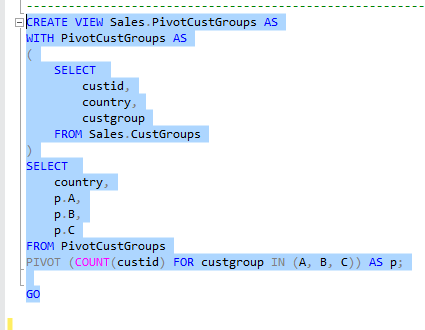
\includegraphics[width=10cm]{./Imagenes/5img1} 
	\end{center}
\textbf{}\\
Paso 4. Haga clic en Ejecutar. Este código crea una vista llamada Sales.PivotCustGroups.

\begin{center}
	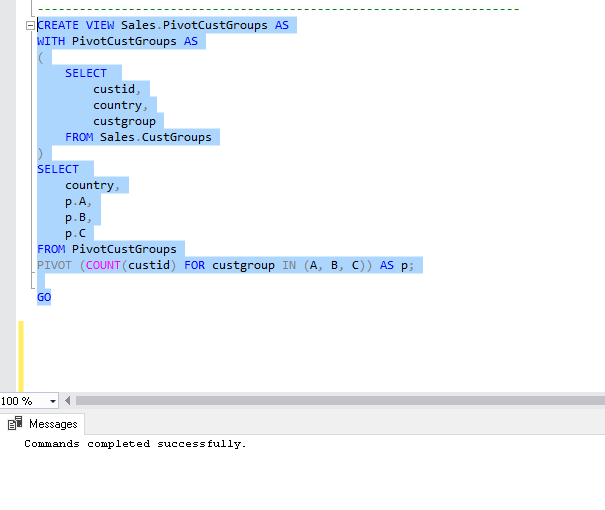
\includegraphics[width=10cm]{./Imagenes/5img2} 
\end{center}
\textbf{}\\
\textbf{}\\
\textbf{}\\
\textbf{}\\
\textbf{}\\
Paso 5. En el panel de consulta, escriba la siguiente consulta después del código T-SQL proporcionado:
\begin{center}
	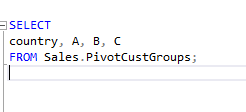
\includegraphics[width=6cm]{./Imagenes/5img3} 
\end{center}
\textbf{}\\
Paso 6. Resalte la consulta escrita y haga clic en Ejecutar.
\begin{center}
	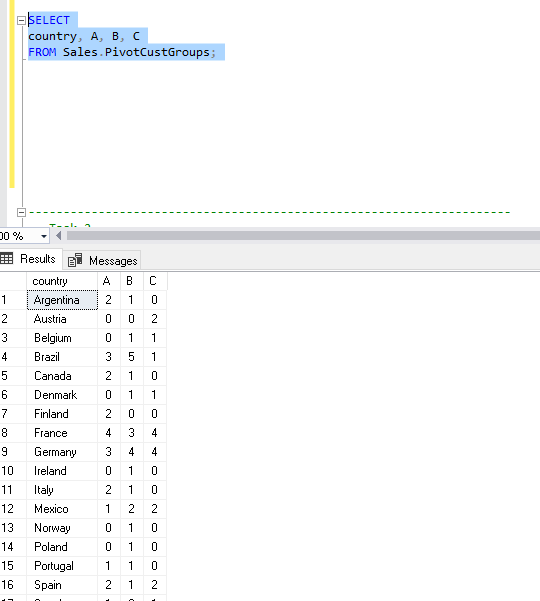
\includegraphics[width=10cm]{./Imagenes/5img4} 
\end{center}
\textbf{}\\
\textbf{}\\
\textbf{}\\
\textbf{}\\
\textbf{}\\
\textbf{}\\
\textbf{}\\
\textbf{}\\
\textbf{}\\
\textbf{}\\
\textbf{}\\
\textbf{}\\
\textbf{}\\
\textbf{}\\

\textbf {Tarea 2: escriba una instrucción SELECT para recuperar una fila para cada país y cliente grupo}
\textbf{}\\
\textbf{}\\
Paso 1. En el panel de consulta, escriba la siguiente consulta después de los descriptores de la Tarea 
\textbf{}\\
\textbf{}\\
SELECT\\
custgroup,\\
country,\\
numberofcustomers\\
FROM Sales.PivotCustGroups\\
UNPIVOT (numberofcustomers FOR custgroup IN (A, B, C)) AS p;
\textbf{}\\
\textbf{}\\

Paso 2. Resalte la consulta escrita y haga clic en Ejecutar.
\begin{center}
	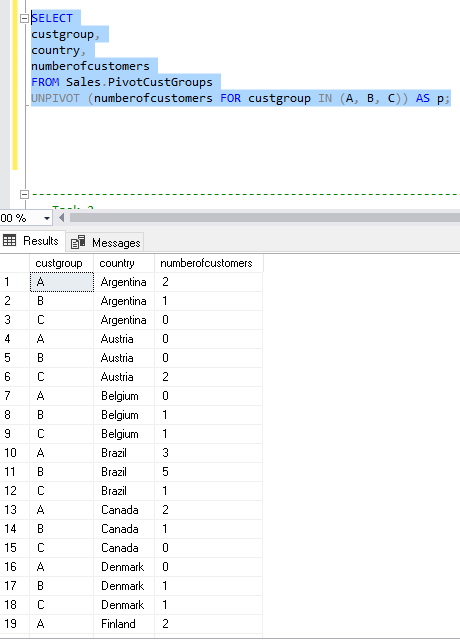
\includegraphics[width=11cm]{./Imagenes/5img5} 
\end{center}
\textbf{}\\
\textbf{}\\
\textbf {Tarea 3: Eliminar las vistas creadas}
\textbf{}\\
\textbf{}\\
- Resalte la instrucción T-SQL proporcionada después de la descripción de la Tarea 3 y haga clic en Ejecutar.
\begin{center}
	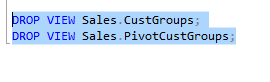
\includegraphics[width=11cm]{./Imagenes/5img6} 
\end{center}














	


 

\end{flushleft}